\documentclass{article}
\usepackage{tikz}

\begin{document}

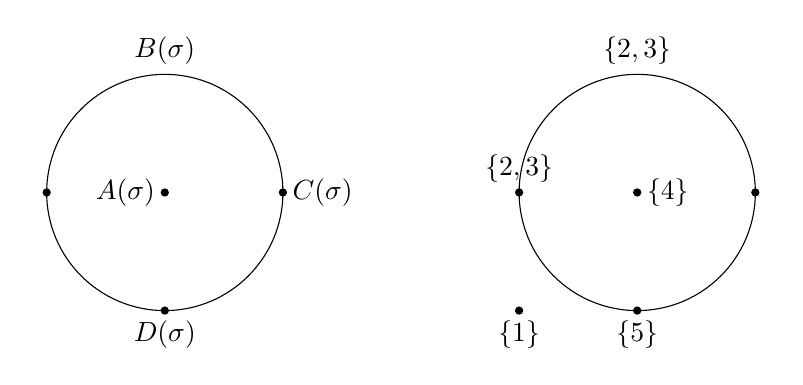
\begin{tikzpicture}[scale=1.5]
    % Draw the circles
    \draw (0,0) circle (1);
    \draw (4,0) circle (1);

    % Label the circles
    \node at (0,1.2) {$B(\sigma)$};
    \node at (4,1.2) {$\{2,3\}$};

    % Label the points on the first circle
    \fill (0,0) circle (1pt) node[left] {$A(\sigma)$};
    \fill (1,0) circle (1pt) node[right] {$C(\sigma)$};
    \fill (-1,0) circle (1pt) node[left] {};
    \fill (0,-1) circle (1pt) node[below] {$D(\sigma)$};

    % Label the points on the second circle
    \fill (4,0) circle (1pt) node[right] {$\{4\}$};
    \fill (3,0) circle (1pt) node[above] {$\{2,3\}$};
    \fill (5,0) circle (1pt) node[right] {};
    \fill (4,-1) circle (1pt) node[below] {$\{5\}$};
    \fill (3,-1) circle (1pt) node[below] {$\{1\}$};
\end{tikzpicture}

\end{document}